\documentclass[UTF8]{ctexart}
\usepackage{subfiles}  

%下面的语句, 引入你的头部设置文件
\usepackage{C:/phpStorm_proj/02_myself_ID_EGO/+100_latex_all_math_sel/myPreamble} 
%必须是绝对路径,才能让各个tex在单独编译时使用到

\title{方法论}


%---------------------------------


\begin{document}
\tableofcontents % 生成目录
\date{} % 若不写这句, 则默认也会渲染出日期, 所以我们要手动赋空值
\maketitle  %这行代码, 让你前面的 title, author, date生效

\section{几何意义 和 物理意义, 本质上是一回事}

一旦碰到较抽象难懂的新概念或定理, 如何搞定? \\
- 看推导过程.\\
- 弄懂它的几何意义, 或物理意义. 几何上说得通,物理上也就说得通,因为几何意义和物理意义本质上是一回事. 因为物理决定着几何结构的存在. n亿年过去了, 不符合物理规律的物质几何空间早就灭亡了. 数学家和物理学家所研究的,只是一头大象的不同部分. \\


\section{真理总是简单的和直观的}

真理总是简单的和直观的. 不管多么复杂高深的数学理论,总有其直观的中心思想. 在数学中再没有别的什么东西,能比几何图形更容易进入人们的脑海了.  \\
数学教育家波利亚曾经说: 一个长的证明常常取决于一个中心思想,而这个思想本身却是直观的和简单的.\\

事实上, 很多数学家都是先利用几何直观, 猜测到某些结果, 然后才补出逻辑上的证明的.\\
华罗庚说过: \textbf{``数缺形"时少直观, ``形少数"时难入微;} ``数形结合"百般好, 割裂分家万事休. \\
抽象和形象是相辅相成,缺一不可的.\\


\section{``线性"问题 and ``非线性"问题}

我们常说的``一次方程"和``一次函数",都属于``线性方程 Linear Equation" 和 ``线性函数 Linear Function. \\
\textbf{现实生活中的数学问题, 无非分为两类: 一类线性问题,一类非线性问题.} 线性问题是研究最久、理论最完善的. 而\textbf{``非线性问题", 则可以在一定基础上转化为``线性问题"来求解.  比如, 微积分学的基本思想, 就是``以直代曲",局部地以``切线"代替``曲线".} 于是,在某种条件下,微分方程就可以近似地变成``线性代数方程组".\\

因此, 你在遇到一个具体问题时, 首先要判断它是``线性"还是``非线性"的. 其次, 若是``非线性问题", 就考虑应如何转化为``线性问题"来解决. \\


\section{不过原点的直线, 不满足线性代数里, 对线性函数的``比例性"的要求}

线性代数里面的``线性", 主要意思就是线性空间里的``线性变换"(映射, 类似函数的概念, 把输入变成另一种输出).\\

函数 f(x)= kx+b (k,b 是不变量),称为一元线性函数. 如果 b=0, 则这个函数的外观就变成 f(x)= k的形式了,这是一条过原点的直线.\\

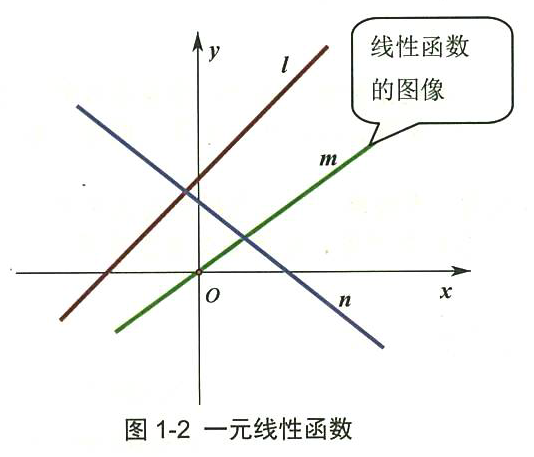
\includegraphics[width=0.4\textwidth]{img/0111.png}\\

严格说来,只有过``原点"的最简单的直线 f(x) = kx, 才被称为一元线性函数.\\

因为\textbf{虽然 f(x)=kx+b 是线性函数, 但它却不满足``线性代数"里所指的``线性"含义. 因为不过原点的直线, 不满足线性代数里, 对线性函数的``比例性"的要求.}\\

\textbf{线性函数, 其几何意义是: 它表示为一条直线. 那么其代数意义呢? 最基本的意义只有两条: ``可加性"和``比例性". }\\

【可加性】:\\
即: 如果函数 f(x) 是线性的, 则有:
\begin{align*}
	\boxed{
	f\left( x_1+x_2 \right) =f\left( x_1 \right) +f\left( x_2 \right)	
	}
\end{align*}

\textbf{其意思就是一句话: 和后的函数, 等于函数后的和.} \\
\textbf{物理意义就是说: 因变量``叠加后"的作用结果, 就等于各个因变量``独自作用结果"的叠加. 即: 先结合, 再做函数变形. 等于 先各自做函数变形, 再结合.}\\


【比例性(数乘)】:\\
也叫做齐次性、数乘性, 或均匀性. 即: 如果函数 f(x) 是线性的, 则有:
\begin{align*}
	\boxed{
	f(kx) = k \cdot f(x)	
	}
\end{align*}

一句话: \textbf{先做比例变化, 后做函数变换, 等于先做函数变换,后做比例变化.}\\
\textbf{物理意义是说: 对因变量做缩放时,函数对因变量的作用结果, 也会同等比例地缩放.} \\

\textbf{而对于不经过原点的直线 f(x)=ax+b 而言, 就不满足此``比例性".} 因为: $f(kx) = akx+b$, 而$k\cdot f(x)=akx+kb$, 所以 $f(kx) \neq k \cdot f(x)$. 因此严格地讲, f(x)=ax+b 不能再叫``线性函数"了. \textbf{或者说,线性代数的``线性变换", 不直接研究坐标系的移动.}\\

可加性与比例性组合在一块, 就是``线性"的全部意义了. 即有:
\begin{align*}
f\left( k_1x_1+k_2x_2 \right) =k_1f\left( x_1 \right) +k_2f\left( x_2 \right) \ \ ←\ k_1,k_2\text{为常数}
\end{align*}
\textbf{一句话: 线性组合的函数,等于函数的线性组合。}这里面既有``缩放"又有``叠加"的物理含义.\\

在物理上, 线性函数的\textbf{``可加性"表明: 函数所描述的事物, 具有累加性. 即: 所有起因的累加, 所导致的结果, 完全等于``每个起因独自所引起的结果"的累加。}\\
\textbf{是否满足``可加性", 就界定了它所描述的事物, 到底是``线性"的, 还是``非线性"的.}\\


比例性是啥物理含义呢? \textbf{比例性又名``齐次性", 说明没有初始值。没有输入信号时, 输出也没有; 有几倍的输入量, 就刚好就有几倍的输出量.}



\section{y=Kx 所做的动作, 就是将一个向量x, 通过矩阵K, 映射变换为另一个新向量y. 矩阵K, 就相当于一个``函数"的作用.}

$
\left\{ \begin{array}{l}
	y_1=k_{11}x_1+k_{12}x_2+...+k_{1n}x_n\\
	y_2=k_{21}x_1+k_{22}x_2+...+k_{2n}x_n\\
	...\\
	y_m=k_{m1}x_1+k_{m2}x_2+...+k_{mn}x_n\\
\end{array} \right. \ ←k_{11},...,k_{mn}\ \text{不是变量,而是系数}
$\\

如上式, 这m个n维(n元)线性函数, 都是齐次函数. 他们全部过原点. \\
线性齐次函数, 形如 $	y=k_{1}x_1+k_{2}x_2+...+k_{n}x_n$, \textbf{这个式子中, 每项里的变量x出现的次数, 都是一次的(没有常数项),整齐划一,故此称为``齐次"的.} 全称为``n元线性齐次函数". \\

上式, 可等价写成: 
$
\left| \begin{array}{l}
	y_1\\
	y_2\\
	...\\
	y_m\\
\end{array} \right|=\left[ \begin{matrix}{l}
	k_{11}&		...&		&		k_{1n}\\
	...&		&		&		\\
	&		&		&		\\
	k_{m1}&		&		&		k_{mn}\\
\end{matrix} \right] \left| \begin{array}{l}
	x_1\\
	x_2\\
	...\\
	x_n\\
\end{array} \right|
$ \\

并可进一步简写成: y=f(x) = Kx \\
即:
$
y=\left| \begin{array}{l}
	y_1\\
	y_2\\
	...\\
	y_n\\
\end{array} \right|,\ K=\left[ \begin{matrix}
	k_{11}&		...&		&		k_{1n}\\
	...&		&		&		\\
	&		&		&		\\
	k_{m1}&		&		&		k_{mn}\\
\end{matrix} \right] ,\ x=\left| \begin{array}{l}
	x_1\\
	x_2\\
	...\\
	x_n\\
\end{array} \right|
$\\
\vspace{1em} 

\textbf{矩阵, 其实就是线性方程组的``系数". 矩阵, 就核心地代表了``线性变换".}\\
因为 \textbf{y=Kx 所做的动作, 就是将一个向量x, 通过矩阵K, 映射变换为另一个新向量y. 矩阵K, 就相当于一个``函数"的作用. 即, 一个矩阵对应着一种``线性变换"规则.} \\





\end{document}